%%%%%%%%%%%%%%%%%%
% Document class %
%%%%%%%%%%%%%%%%%%

\documentclass[a4paper, 12pt]{article}


%%%%%%%%%%%%
% Packages %
%%%%%%%%%%%%

\usepackage[english]{babel}
\usepackage[noheader]{packages/sleek}
\usepackage{packages/sleek-title}


%%%%%%%%%%%%%%%%%%%%
% Title page setup %
%%%%%%%%%%%%%%%%%%%%

\logo{resources/pdf/logo-uliege.pdf}
\institute{University of Liège}
\title{Securing network with firewalls and NATs}
\subtitle{Step 1: drawing the network}
\author{Maxime \textsc{Meurisse}\\Valentin \textsc{Vermeylen}}
\context{Master in Civil Engineering}
\date{Academic year 2020-2021}


%%%%%%%%%%%%
% Document %
%%%%%%%%%%%%

\begin{document}
	\maketitle
	
	\section{Drawing of the network}
	
	The representation of the network topology is shown in Figure \ref{fig:network.topology}. This figure is in vector format: it is possible to zoom in on it for better reading without loss of quality.
	
	\begin{figure}[H]
	    \centering
	    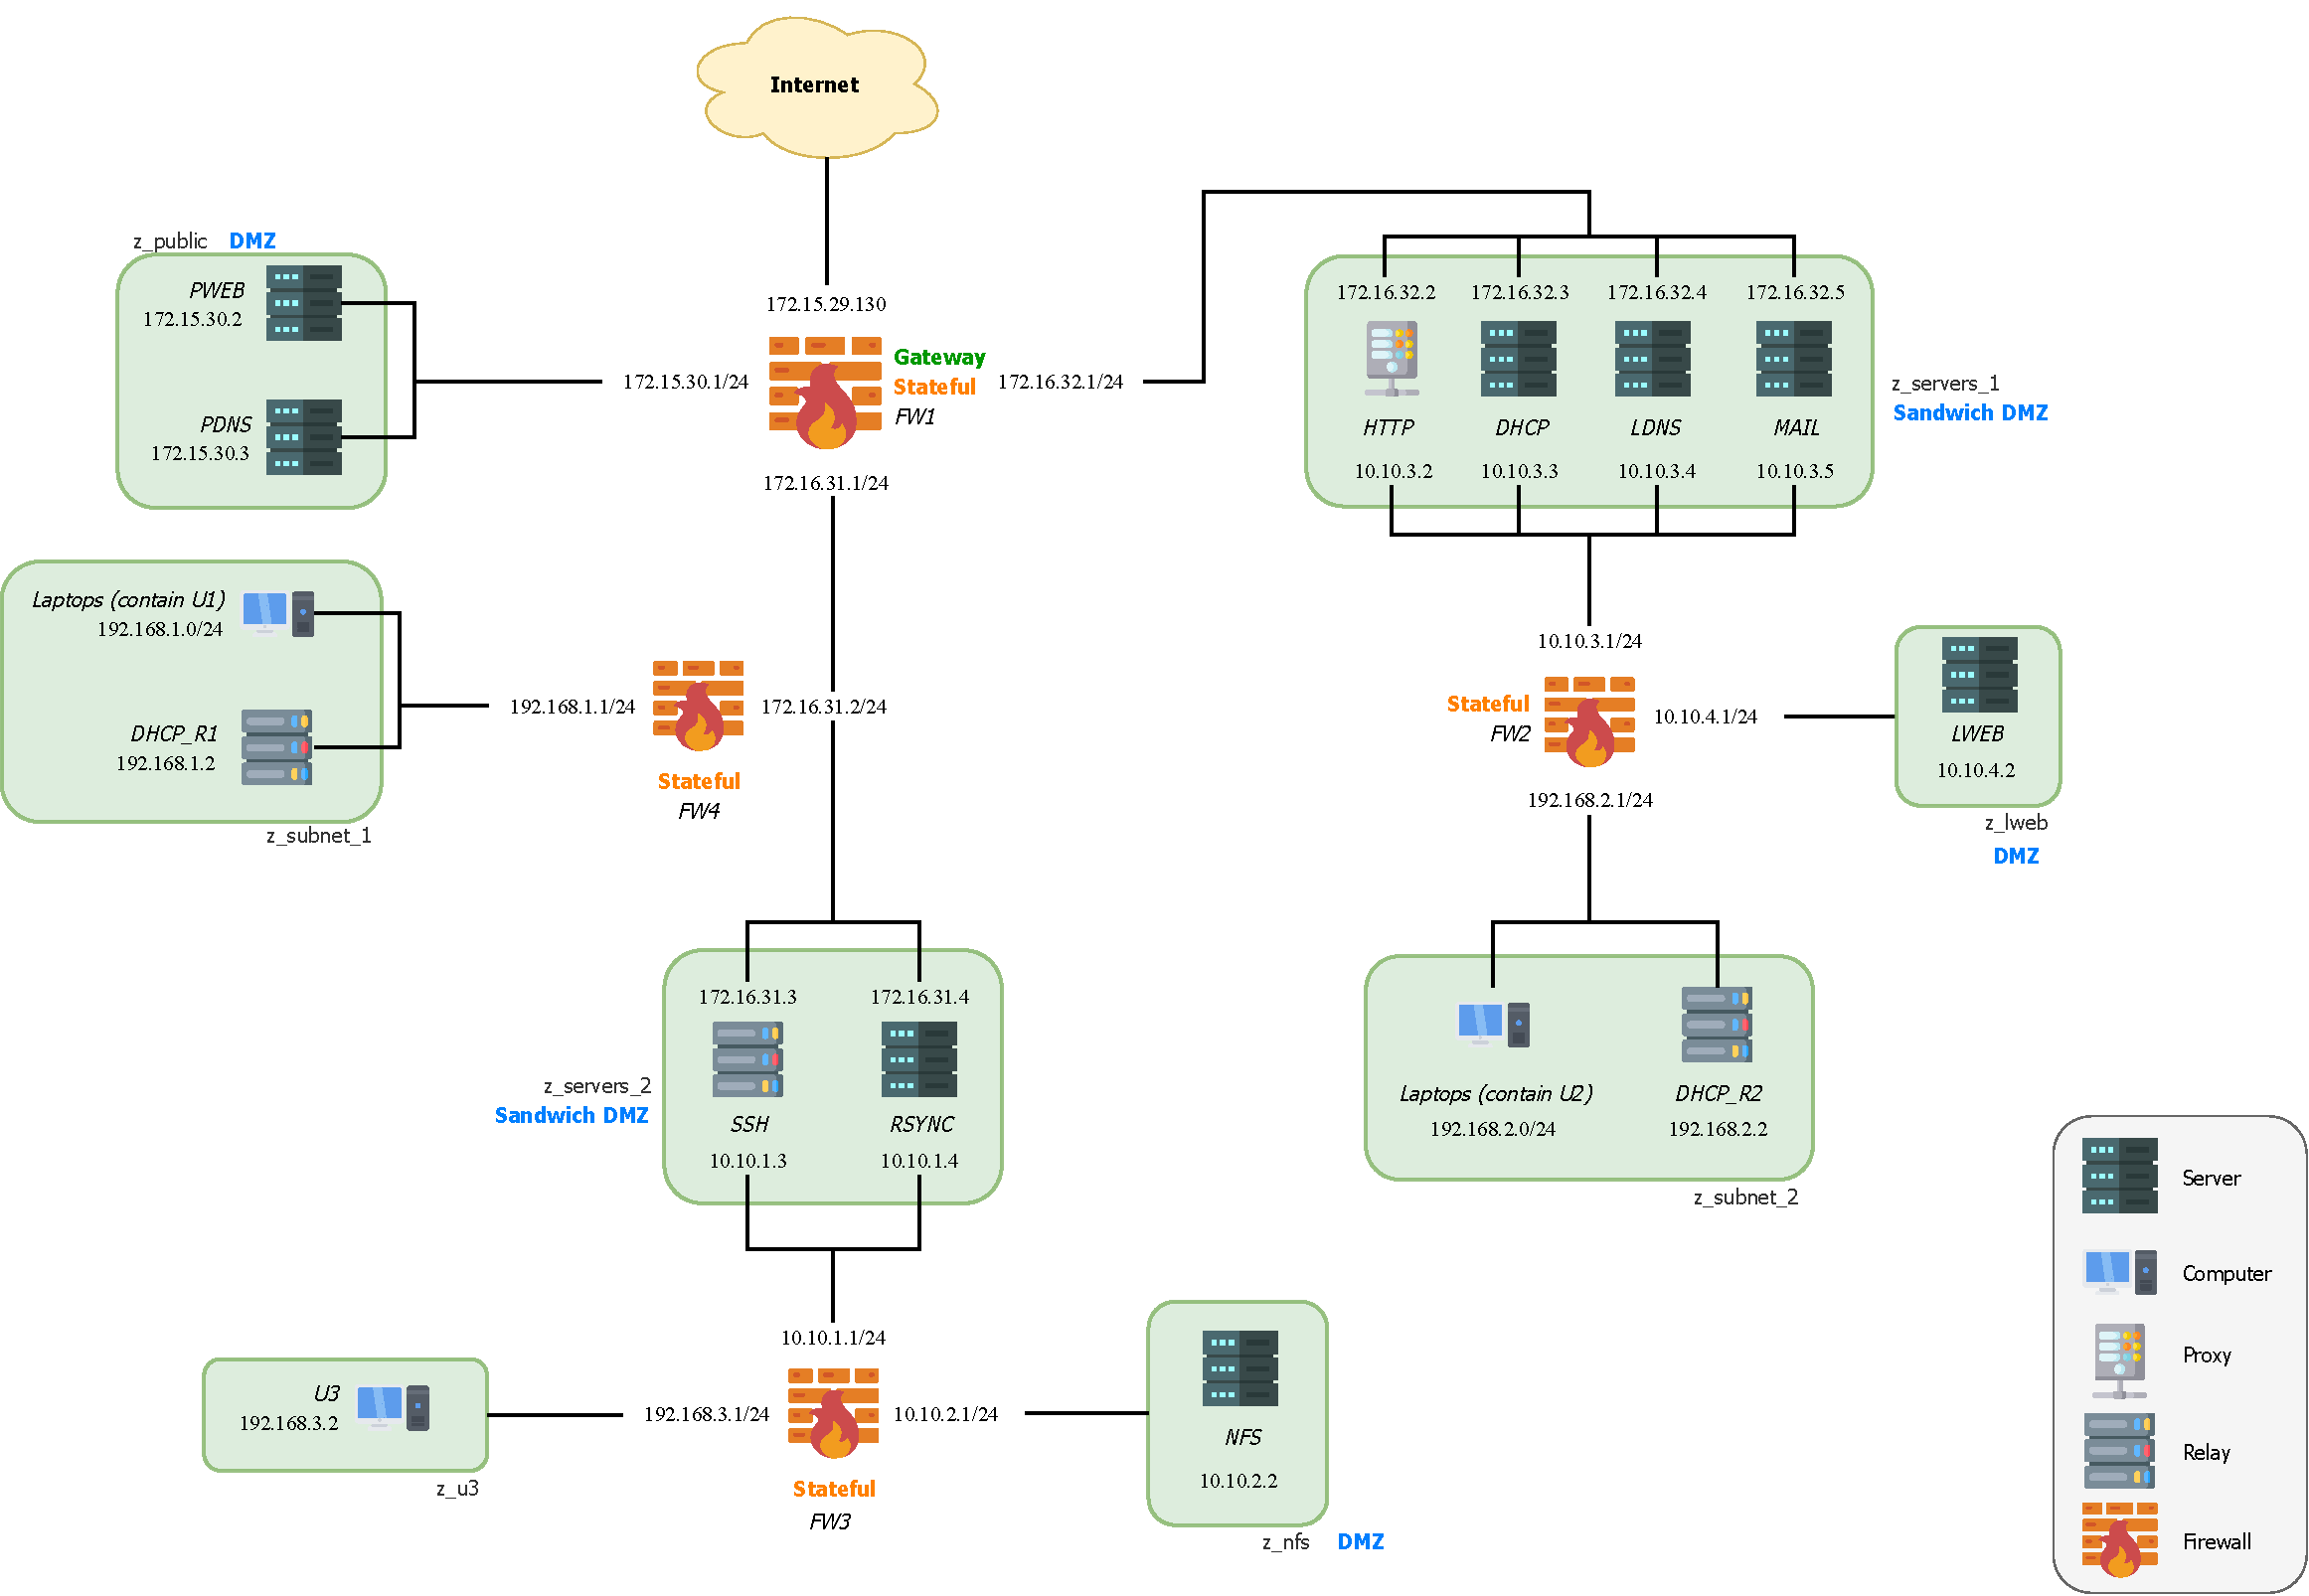
\includegraphics[width=0.9\textwidth]{resources/pdf/topology.pdf}
	    \caption{Topology of the network.}
	    \label{fig:network.topology}
	\end{figure}
	
	\section{Details of the network}
	
	This network is composed of 4 firewalls, 8 zones and several types of machines (servers, proxies, computers and relays).
	
	\subsection{Firewalls}
	
	The 4 firewalls present in the network are \emph{stateful} firewalls.
	
	The firewall \emph{FW1} is a gateway: it acts as a link between the Internet and the company's internal network. A NAT configuration will be necessary on this firewall. The NAT interfaces are: \texttt{172.15.29.130}, \texttt{172.16.32.1/24}, \texttt{172.16.31.1/24} and \texttt{172.15.30.1/24}.
	
	The other firewalls (\emph{FW2}, \emph{FW3} and \emph{FW4}) are \enquote{classical} firewalls that do not act as NATs.
	
	\subsection{Zones}
	
	The network is composed of 8 zones: \emph{z\_public}, \emph{z\_servers\_1}, \emph{z\_servers\_2}, \emph{z\_lweb}, \emph{z\_subnet\_1}, \emph{z\_subnet\_2}, \emph{z\_u3} and \emph{z\_nfs}. Each zone has been defined by grouping together devices that have the same IP address prefix.
	
	The \emph{z\_public}, \emph{z\_lweb} and \emph{z\_nfs} zones are \emph{DMZ}. The \emph{z\_servers\_1} and \emph{z\_servers\_2} zones are \emph{sandwich DMZ} (because zones are between 2 firewalls). These zones are considered are DMZ because they are connected neither to the Internet, or the internel network. The internal network is represented by \emph{z\_subnet\_1}, \emph{z\_subnet\_2} and \emph{z\_u3} zones.
	
	\subsubsection{Zone classification}
	
	For each firewall, zones are classified from more secured to less secured.
	
	\begin{itemize}
	    \item \emph{FW1}
	    \begin{itemize}
	        \item \emph{z\_servers\_1}
	        \item \emph{z\_public}
	    \end{itemize}
	    \item \emph{FW2}
	    \begin{itemize}
	        \item \emph{z\_subnet\_2}
	        \item \emph{z\_lweb}
	    \end{itemize}
	    \item \emph{FW3}
	    \begin{itemize}
	        \item \emph{z\_nfs}
	        \item \emph{z\_u3}
	    \end{itemize}
	    \item \emph{FW4}
	    \begin{itemize}
	        \item \emph{z\_subnet\_1}
	        \item \emph{z\_servers\_2}
	    \end{itemize}
	\end{itemize}
	
	We have considered that the deeper a zone is in the network (\emph{i.e.} behind more firewalls), the more secure it is.
	
	\subsection{Devices}
	
	The network is composed of several devices. The type of each device is represented by its icon. Note that in zones \emph{z\_subnet\_1} and \emph{z\_subnet\_2}, company computers (\enquote{Laptops}) cannot have the same IP address as the DHCP relay in the same zone.
\end{document} 
